\subsection{\textit{CyberCode}}
\label{sec:cybercode}
	
	Em \cite{rekimoto} é apresentado uma proposta de utilização de marcadores baseados em códigos
	bidimensionais, denominado de CyberCode. Nesta aplicação as informações são codificadas em um
	padrão bidimensional para ser reconhecido por dispositivos de baixo desempenho. As informações
	correspondente aos marcadores são armazenados em um banco de dados, possibilitando assim a
	alteração dos dados de forma dinâmica, sem a necessidade de alterar o marcador. A
	figura~\ref{fig:cybercode} mostra um exemplo do marcador CyberCode.
	
	\begin{figure}[htb]
		\centering 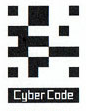
\includegraphics[scale=1]{figuras/cap2/cybercode.png}
		\caption{\textit{Exemplo de um marcador CyberCode \cite{rekimoto}.}}
		\label{fig:cybercode} 
	\end{figure} 
	 
	O uso dos mesmos pode ser combinado com outras tecnologias de rastreamento, com o objetivo de
	auxiliar o usuário na navegação em um ambiente específico. Desta maneira, eles seriam
	reconhecidos com o propósito de obtenção da localização do usuário no espaço. Com isso seria
	possível apresentar as informações ao usuário a respeito dos demais locais próximos a ele.
	
	Uma outra proposta para esses marcadores diz respeito a utilização dos mesmos para o mapeamento dos
	dispositivos. A própria equipe construiu um dispositivo de fácil manuseio constituído por uma
	câmera e um visor, denominado de \textit{InfoPoint}. Esse dispositivo capta a imagem correspondente
	ao marcador, acessa um banco de dados para extrair o conteúdo correspondente e apresenta o conteúdo
	correspondente no visor do dispositivo. Através desse dispositivo, o usuário é capaz de selecionar
	um marcador específico e transferir dinamicamente o conteúdo relativo a esse CyberCode para um outro
	marcador.
	
	\subsubsection{Aplicado à computação ubíqua}
	 
	A integração desse projeto com a computação ubíqua ocorre através da utilização de uma mesa
	digital. Sobre esta são acopladas câmeras com o propósito de reconhecer os objetos
	distribuídos em sua superfície. Após o reconhecimento de um novo dispositivo marcado por um
	CyberCode são apresentadas as informações correspondente ao objeto reconhecido. 
	
	Também é apresentada a utilização da mesa através da integração com um \textit{notebook}. O
	\textit{notebook} é reconhecido através do seu marcador associado, posteriormente é feita uma busca
	das informações relativas ao dispositivo, como por exemplo seu endereço~\textit{IP} e o
	posicionamento relativo a mesa digital. Desta forma, o \textit{notebook} estará integrado com a
	rede local juntamente com os objetos físicos reconhecidos pela mesa.
	
	Essa integração possibilita uma troca de informações livre entre os dispositivos. No exemplo
	anterior, o recurso de tela do \textit{notebook} foi estendido para a mesa digital. Isso
	possibilita com que o usuário utilize os recursos da mesa digital para interagir com o
	\textit{notebook}. Por exemplo, caso o usuário sinta a necessidade de mover o cursor do
	\textit{notebook}, ele poderá utilizar a sensibilidade da mesa para mover o cursor dentro do espaço
	delimitado como extensão da tela do \textit{notebook}.
	
